\documentclass[runningheads,12pt]{llncs}
\usepackage{graphicx}
\usepackage{todonotes}
\usepackage{fancyhdr}
\usepackage{lipsum}
\usepackage{tabularx}
\usepackage{array}
\usepackage{longtable}
\usepackage[T1]{fontenc}
\usepackage[provide=*,english,polish]{babel}

\newcolumntype{C}[1]{>{\centering\arraybackslash}m{#1}}

\setcounter{tocdepth}{4}
\setcounter{secnumdepth}{4}
\renewcommand{\headrulewidth}{0pt}

\begin{document}

\title{Współdzielenie kodu w mikroserwisach} \subtitle{}

\author{Artem Romanenko \ Student number: S32237 \inst{}}
\authorrunning{ }
\titlerunning{Your thesis title abbreviated.}
\institute{\textbf{Polish-Japanese Academy of Information Technology} \ Promotor pracy magisterskiej: Krzysztof Barteczko, PhD}

\thispagestyle{fancy}

\begin{figure}[t!]
    \centering
    
\includegraphics[width=\linewidth]{images/Logo_EN_1.png}
    \label{fig:my_label}
\end{figure}

\selectlanguage{english}
\cfoot{ Warsaw, \today}

\clearpage

\makeatletter
\renewcommand*\l@author[2]{}
\renewcommand*\l@title[2]{}
\makeatletter

\selectlanguage{english}
\begin{abstract}
Rapid development and adoption of microservices architecture in last few years changed the world of Informatics. Microservices architecture has many advantages, such as flexibility, fast and comfortable deployment, and easy maintenance. However, this architecture also causes new challenges, such as code duplication and complicated code management. In my master's thesis, I've carried on deep and detailed analysis of all available approaches to manage shared code in system of microservices. In my work, I want to compare all available approaches of code share code in system of microservices using literature sources and prepared code laboratory, also to define cases in which it is better to choose one or another approach. In my practical part, I want to present my own approach to sharing code that will combine the advantages of all existing solutions and provide the best performance and code comfort for developer in code management. At the end of my work, I will place comparison of my solution with existing solutions using prepared performance tests.
\keywords{Microservices Architecture \and Code Sharing \and Performance.}
\end{abstract}

\newpage

\selectlanguage{polish}
\begin{abstract}
Bez wątpienia mogę powiedzieć, że szybki rozwój i przyjęcie architektury mikroserwisowej w ostatnich latach zmieniły świat informatyki. Uważam, że architektura mikroserwisowa ma wiele zalet, takich jak na przykład elastyczność, prostota wdrożenia i utrzymania. Natomiast powoduje nowe wyzwania dla programistów, takie jak do przykładu problem duplikacji kodu. W pracy magisterskiej przeprowadziłem dokładną analizę metod i podejść współdzielenia kodu w systemach mikroserwisów, porównanie za pomocą źródeł literaturowych oraz przeprowadzonych badań dostępne podejścia do współdzielenia kodu, zdefiniować przypadki, w których warto wybrać takie lub inne podejście. W części praktycznej zaprezentowałem własne nowoczesne rozwiązanie, które połączyło zalety istniejących rozwiązań, wydajność oraz komfort zarządzania kodem. Na końcu umieściłem porównanie mojego rozwiązania z istniejącymi za pomocą przygotowanych testów wydajnościowych.
\keywords{Architektura mikrousług \and Współdzielenie kodu \and Wydajność.}
\end{abstract}

\newpage

\tableofcontents

\newpage

\section{Wstęp}

\subsection{Zakres pracy}
W pracy magisterskiej przeprowadzono dokładną analizę metod i podejść do współdzielenia kodu w systemach mikroserwisów. Zakres tej pracy zawiera porównanie między architekturą monolitową a mikroserwisową, identyfikację typów obiektów wykorzystywanych w kodzie współczesnych aplikacji, analizę dostępnych metod i podejść do współdzielenia kodu, IDL, SDK oraz biblioteki, a także praktyczną implementację aplikacji wspierającej nowatorskie podejście do współdzielenia kodu Serverless.

\subsection{Motywacja}
Główną motywacją do napisania pracy było rosnące we współczesnych czasach zainteresowanie mikroserwisowym podejściem do architektury, które ma wiele zalet, takich jak elastyczność, łatwość wdrożenia i utrzymania na produkcji, możliwość łatwej i szybkiej naprawy problemów na produkcji, natomiast również powoduje nowe wyzwania, takie jak problem duplikacji kodu i zapotrzebowanie na współdzielenie kodu między mikroserwisami w systemie.
W mojej pracy chcę przeanalizować, jakie metody współdzielenia kodu są dostępne na rynku, jakie są ich zalety i wady, jakie są najlepsze praktyki we współdzieleniu kodu w systemach mikroserwisów. Chcę porównać bardziej tradycyjne podejścia do współdzielenia kodu, takie jak IDL, SDK, biblioteki, z nowatorskim podejściem do współdzielenia kodu, takim jak Serverless, chcę stworzyć oprogramowanie, które połączy główne zalety tradycyjnych metod współdzielenia kodu z zaletami bardziej nowoczesnych podejść.

\newpage

\subsection{Zawartość pracy}
Praca jest ustrukturyzowana w kilka rozdziałów, przedstawiam krótki opis rozdziałów parcy:
\begin{enumerate}
    \item Wstęp - W tym rozdziale analizuję wady i zalety architektury mikroserwisowej oraz monolitycznej, też analizuję, dlaczego z architektury monolitycznej powstała w ostatich latach architektura mikroserwisowa, robię analizę przypadków w których lepiej użyć architektury monolitycznej a w których architekturę mikroserwisową. Opisuję dlaczego powstało zapotrzebowanie na współdzielenie kodu. Uzasadniam informację przykładami z literatury.
    \item Architektura mikroserwisowa a Monolitowa - W tym rozdziale paracy porównuję mikroserwisy z podejściem monolitycznym, przedstawiam różnice w utrzymaniu i skalowalności, za pomocą źródeł literaturowych.
    \item Analiza dziedziny problemowej - W tym rozdziale przedstawiam kategoryzuję typy obiektów które mogą potrzebować współdzielenia kodu w systemie mikroserwisów, analizuję możliwe wyzwania związane z współdzieleniem poszczególnych typów obiektów, przedstawiam uzasadnienia z literatury.
    \item Analiza metod współdzielenia kodu - W tym rozdziale kompleksowa analiza istniejących metod współdzielenia kodu w systemach mikroserwisów za pomocą źródeł literaturowych kryterium ocenia.
    \item Opis części praktycznej - Zawiera opis przygotowanej w ramach pracy aplikacji która wspomaga nowoczesne rozwiązanie do współdzielenia kodu w systemach mikroserwisów - Server Less rozszerzając możliwości tego rozwiązania.
\end{enumerate}

\newpage

\section{Architektura mikroserwisowa a monolitowa}

Mikroserwisowa infrastruktura, szybko rozwijająca się w ostatnich latach, przyniosła wiele korzyści w świat informatyki. Pozwoliła na tworzenie skalowalnych i elastycznych systemów, ułatwiła utrzymanie takich systemów. Natomiast musimy również uważać przy wyborze architektury na to, że w przypadku mikroserwisów musimy poradzić sobie z kwestią współdzielenia kodu w takim systemie mikroserwisów.

\subsection{Architektura mikroserwisowa}

Na podstawie mojego doświadczenia, podział aplikacji na mniejsze, niezależne usługi przynosi liczne korzyści. Każdy mikroserwis można skalować osobno, co pozwala na poprawę wydajności całego systemu. W sytuacji, gdy pojawia się problem, naprawa jest prostsza, ponieważ wystarczy skupić się na jednej części aplikacji, a nie na całym systemie. Mikrousługi wpływają również na organizację pracy zespołowej. Deweloperzy mogą skupić się na rozwoju pojedynczych mikroserwisów, co ułatwia zarządzanie projektem i zmniejsza ryzyko wystąpienia błędów w innych częściach aplikacji. Ponadto, gdy pojawia się problem, jest on łatwiejszy do zidentyfikowania, a proces naprawy staje się bardziej efektywny. Kolejną zaletą mikrousług, moim zdaniem, jest ich elastyczność pod względem doboru technologii. Dzięki temu, że każdą usługę można tworzyć i zarządzać nią z użyciem różnych narzędzi, istnieje większa swoboda w doborze najlepszych rozwiązań technologicznych do każdej części systemu. Mikrousługi wspierają również skuteczne zarządzanie projektem, ponieważ umożliwiają szybsze wdrażanie nowych funkcji i reagowanie na zmiany. Taki system jest bardziej odporny na awarie, a cały proces utrzymania aplikacji jest prostszy.
\begin{quote}
    "Microservices are small, autonomous services that work together. Let’s break that definition down a bit and consider the characteristics that make microservices different."~\cite[p. 2]{newman2015building}
\end{quote}

Architektura mikrousług przedstawia następujące cechy:

\begin{enumerate}
    \item Modułowość - W przypadku mikroserwisów możemy wdrażać pojedyncze elementy systemu bez wpływu na pozostałe.
    \item Niezawodność - Mikroserwisy są niezawodne, ponieważ błąd w jednej części systemu niekoniecznie będzie miał wpływ na cały system.
    \item Interoperacyjność — Komunikacja za pomocą wymiany danych przez zasoby sieciowe daje nam możliwość połączenia mikroserwisów napisanych w różnych językach i technologiach. W tym przypadku możemy połączyć w jednym systemie kilka technologii i wykorzystać mocne strony każdej z nich.
    \item Równoległy rozwój - Zespoły programistów mogą pracować nad osobnymi mikroserwisami równolegle, bez konfliktów zmian w kodzie.
\end{enumerate}

\subsection{Architektura monolitowa}

Charakterystyka architektury monolitycznej:

\begin{enumerate}
    \item Wdrożnie - Cała aplikacja jest wdrażana jako całość, niepodzielna jednostka. Wszustkie aktualizacje wymagają wdrożenia całej aplikacji.
    \item Kontrola przepływu kodu - Centralny moduł kontroli w aplikacji koordynuje sekwencyjne wykonywanie kodu.
    \item Powiązanie - Poszczególne elementy aplikacji są ścisłe powiązane.
    \item Współdzielona pamięć - Wszystkie komponenty oprogramowania mają bezpośredni dostęp do zasobów, co sprzyja ich integracji, natomiast taka konfiguracja może powodować konflikty elementów kodu na poziomie sprzętowym i trudności ze skalowaniem. \cite{sharma2023monolithic}
\end{enumerate}

\subsection{Porównanie}

\begin{quote}
    "I should call out that microservices are no free lunch or silver bullet, and make for a bad choice as a golden hammer. They have all the associated complexities of distributed systems."~\cite[p. 11]{newman2015building}
\end{quote}

Zalety architektury monolitycznej:

\begin{itemize}
    \item Czas napisania – Dla małych i średnich projektów umożliwia szybsze napisanie kodu bez potrzeby zarządzania komunikacją między mikroserwisami w systemie.
    \item Łatwość wdrożenia – Wdrożenia kodu w przypadku architektury monolitycznej są mniej skomplikowane.
    \item Proste testowanie – O wiele łatwiejsze jest testowanie aplikacji monolitycznej dzięki ścisłej integracji wszystkich komponentów. Testy jednostkowe i integracyjne można w prosty sposób przeprowadzać w ramach pojedynczej bazy kodu.
    \item Skalowalność – Zapewnia odpowiednią skalowalność dla niewielkich rozwiązań poprzez replikację całej aplikacji.
\end{itemize}

Zalety architektury mikroserwisowej:

\begin{enumerate}
    \item Skalowalność - Mikroserwisy umożliwiają niezależne skalowanie, optymalizując wykorzystanie zasobów i zapewniając wydajność systemu.
    \item Równoległa praca - Architektura mikroserwisowa pozwala na równoległy rozwój kilku elementów systemu bez konfliktów, co prowadzi do szybszego rozwoju.
    \item Elastyczność - Każdy mikroserwis może być napisany w języku najbardziej pasującym do jego konkretnej funkcji, daje to możliwość użycia mocnych stron każdej z wielu dostępnych technologii.
    \item Debugowanie - Rozwiązywanie problemów w mikroserwisach jest prostsze, każdy osobny mikroserwis jest niewielki i prosty w analizie.
    \item Bezpieczeństwo - Mikroserwisy ułatwiają ochronę danych. Każda usługa ma swoją bazę danych, co utrudnia hakerom dostanie się do danych.~\cite{sharma2023monolithic}
\end{enumerate}

Wybór między architekturą monolityczną a mikroserwisową zależy od wielu faktorów, takich jak rozmiar projektu, zapotrzebowanie na ciągły rozwój, wymagania dotyczące skalowalności oraz kompetencje i doświadczenia zespołu. Architektura monolityczna lepiej pasuje dla małych i mniej skomplikowanych projektów natomiast mikroserwisowa oferuje benefity w przypadku wykorzystania w większych, bardziej skomplikowanych systemach.

\newpage

\section{Analiza dziedziny problemowej}

Celem niniejszej pracy magisterskiej jest zgłębienie tematu współdzielenia obiektów w systemach mikroserwisów oraz zrozumienie wyzwań i możliwości związanych z tym zagadnieniem. Praca ma na celu analizę różnych strategii, narzędzi i metodyk, które mogą pomóc w efektywnym i bezpiecznym współdzieleniu danych i obiektów w skali mikroserwisowej architektury.

\subsection{Typy obiektów w aplikacjach mikroserwisowych}

Postanowiłem rozpocząć analizę dziedziny problemowej od tego że za pomocą źródeł literaturowych zidentyfikuję typy obiektów oraz dokonać analizy tego, które z nich mogą wymagać współdzielenia w systemach mikroserwisów.

\begin{enumerate}
    \item DTO (Data Transfer Object) - Takie obiekty są specjalnie przeznaczone do obsługi przesyłania danych między elementami systemu mikroserwisów, są lekkie i nie zawierają logiki biznesowej, dlatego współdzielenie takich obiektów jest jak najbardziej zalecane ponieważ zapewniają spójność danych po obu stronach komunikacji oraz zmniejsza ilość błędów w przypadku rozwoju lub utrzymania aplikacji.
    \item Model (lub Encja) - Najczęściej są logicznie powiązane z tabelami w bazie danych, ze względu na to że we współczesnych czasach za dobrą praktykę jest uważane podejście w którym jeden mikroserwis jest powiązany z maksymalnie jedną bazą danych, współdzielenie tego typu obiektów nie jest zalecane.
    \item Wyjątek (Exception) - Zalecanym jest współdzielenie informacji o wyjątkach w systemie mikroserwisów tym samym tworząc jednolitą obsługę błędów w systemie. Logika związana z obsługą błędów, w przypadku podobności w kilku serwisach też jest dobrym kandydatem do współdzielenia. Taka standaryzacja w systemie mikroserwisów sprawia że łatwiej później znaleźć źródło błędu i naprawić go.
    \item Walidatory - W przypadku współdzielenia walidatorów w systemie mikroserwisów można zapewnić integralność danych w całym systemie oraz zmniejszyć duplikację kodu, również standaryzacja walidacji obiektów w systemie zmniejsza ilość ewentualnych problemów w trakcie ewolucji i rozwoju mikroserwisów w przyszłości, współdzielenie takich obiektów jest dobrą praktyką i jest zalecane.
    \item Serwisy - W przypadku logiki która powtarza się w dwóch i więcej serwisach zalecanym jest współdzielenie takiego serwisu za pomocą najlepiej w tym przypadku pasującej metody, zmniejsza to duplikację kodu natomiast zwiększa czytelność i spójność kodu w systemie mikroserwisów, zmniejsza ilość ewentualnych problemów w trakcie ewolucji i rozwoju kodu.
\end{enumerate}

Musimy zdawać sobie sprawę, że mimo tego, iż współdzielenie kodu daje nam wiele korzyści, nadmiarowe współdzielenie kodu może spowodować problemy i pogorszyć jakość oraz zrozumiałość naszego kodu, utrudnić testowanie, spowodować powstanie błędów kaskadowych, czyli sytuacji, kiedy błąd w jednym źródle powoduje problemy od razu w wielu miejscach, oraz utrudnić utrzymanie systemu. Należy zawsze używać współdzielenia ostrożnie i podejmować decyzję w każdym konkretnym przypadku współdzielenia.

\newpage

\subsection{Kryteria porównania i analizy metod współdzielenia kodu}

Po przeprowadzeniu dogłębnej analizy tematu i między innymi źródeł literaturowych, takich jak ~\cite{newman2015building}, ~\cite{richardson2018microservices}, ~\cite{nygard2008release}, ~\cite{kleppmann2017designing} mogę zdefiniować kryteria porównania metod współdzielenia kodu w systemach mikroserwisów jako następujące:
% AI
\begin{enumerate}
    \item Komunikacja - Metoda współdzielenia obiektów powinna uwzględniać efektywną komunikację między serwisami. Ważne jest, aby obiekty były dostępne w sposób, który minimalizuje opóźnienia i obciążenie sieci. Dobre rozwiązania mogą obejmować użycie asynchronicznej komunikacji, takiej jak kolejki wiadomości, czy też bezpośrednie zapytania między serwisami.
    \item Izolacja - Metoda współdzielenia obiektów powinna zapewniać odpowiednią izolację między serwisami. Każdy serwis powinien mieć kontrolę nad swoimi własnymi obiektami i nie powinien być zależny od innych serwisów. To pozwala na większą elastyczność i umożliwia niezależny rozwój i skalowanie serwisów.
    \item Bezpieczeństwo - W przypadku współdzielenia obiektów, istotne jest zapewnienie odpowiedniego poziomu bezpieczeństwa. Dostęp do obiektów powinien być kontrolowany i zabezpieczony w sposób, który zapobiega nieautoryzowanemu dostępowi. Mechanizmy uwierzytelniania i autoryzacji powinny być odpowiednio wdrożone, aby zapewnić bezpieczne współdzielenie obiektów.
    \item Skalowalność - Metoda współdzielenia obiektów powinna być skalowalna. System powinien być w stanie efektywnie obsługiwać rosnącą liczbę żądań i zapewniać odpowiednią wydajność. Współdzielenie obiektów powinno być projektowane w taki sposób, aby możliwe było łatwe skalowanie poszczególnych serwisów bez wpływu na cały system.
    \item Wersjonowanie - Ważne jest również odpowiednie zarządzanie wersjami obiektów, szczególnie w środowisku mikroserwisów, gdzie różne serwisy mogą używać różnych wersji obiektów. Metoda współdzielenia obiektów powinna uwzględniać zarządzanie wersjami i umożliwiać aktualizacje w sposób kontrolowany i bezpieczny.
\end{enumerate}

\newpage

\section{Analiza metod współdzielenia kodu}

We współczesnych czasach współdzielenie kodu jest niezbędne w skomplikowanych systemach mikroserwisów, w tym rozdziale pracy porównuję istniejące podejścia do współdzielenia kodu oraz porównam je za pomocą zdefiniowanych w poprzednim rozdziale kryteriów. Głównym celem jest zdefiniowanie najlepszych praktyk współdzielenia kodu, zdefiniować, które podejście najbardziej dopasowane do współdzielenia konkretnych typów obiektów, zdefiniowanych powyżej w tej pracy oraz porównanie wydajności i możliwości skalowania w przypadku każdego z podejść za pomocą przygotowanych programistycznych testów wydajnościowych.

\subsection{Metody współdzielenia kodu z opisem}

Za pomocą źródeł literatury oraz własnego doświadczenia zdefiniowałem dostępne na dzień dzisiejszy podejścia:

\begin{enumerate}
    \item Interface definition languages - do IDL należą wiele popularnych technologii, Protocol buffers, Avro IDL, Open API. ~\cite{wiki:interface_description_language}
    \item Biblioteki kodu - najbardziej oczywiste podejście, które daje możliwość współdzielenia wszystkich rodzajów obiektów w aplikacji.
    \item Biblioteki klienckie - podejście które polega na udostępnieniu za pomocą biblioteki kodu zestawu obiektów potrzybnych do kmonikacji z narzedziem zewnętrznym, takim jak, na przykład konsola AWS.
    \item Wyniesienie kodu do osobnego REST serwisu - podejście polega na przechwytywaniu i udostępnieniu wspólnej logiki poprzez utworzenie osobnego mikroserwisu.
    \item Serverless - nowoczesne podejście do pisania kodu i przetwarzania informacji wykorzystywane w chmurach obliczeniowych. Pozwala na uruchamianie kawałków kodu, metod i funkcji niezależnie, bez warstwy zarządzania aplikacją, a także na uruchamianie kodu bez konieczności zarządzania podstawową infrastrukturą. ~\cite{ibm_serverless}
\end{enumerate}
% AI
Pryncypia działania poszczególnych metod współdzielenia kodu:

Interface definition languages – są powszechnie używane w oprogramowaniu zdalnych wywołań procedur. W takich przypadkach maszyny po obu stronach łącza mogą używać różnych systemów operacyjnych i języków programowania. IDL oferują most pomiędzy dwoma różnymi systemami. Natomiast również mogą być użyte dla generacji obiektów lub kodów w systemach mikroserwisów. Każdy system IDL posiada określony przez twórców język IDL oraz interpretator języka IDL. Interpretator języka IDL przygotowany i dostarczony przez twórców potrafi na podstawie udostępnionych reguł wygenerować kod używając przygotowane pliki IDL. Używając języka IDL możemy przygotować obiekty lub kod zapisany za pomocą języka IDL, a później udostępnić przygotowane pliki IDL nieograniczonej ilości mikroserwisów i na podstawie udostępnionych plików wygenerować w każdym z mikroserwisów kod lub obiekty, które zostaną użyte przez specyficzną logikę konkretnego serwisu dla osiągnięcia konkretnego celu biznesowego. Tworzenie kodu na podstawie plików IDL jest łatwo zautomatyzowane za pomocą narzędzi do budowania aplikacji, takich jak Gradle czy Maven, dlatego możemy używać IDL jako metodę współdzielenia kodu. W trakcie pracy zamierzam sprawdzić skuteczność tej metody, problemy związane z jej użyciem oraz określić przypadki, w których dobrze się nadaje, jak również przypadki, w których lepiej jej nie stosować.

Libraries – biblioteki to w odpowiedni sposób przygotowany kod, który my za pomocą odpowiednich narzędzi możemy łatwo importować i używać jako część innego programu. Program importujący bibliotekę może używać kodu biblioteki tak, jakby to był własny kod programu. Istnieje wiele narzędzi, które wspomagają łatwe i szybkie importowanie i zarządzanie bibliotekami kodu, takie jak Maven czy Gradle. W współczesnych systemach mikroserwisów współdzielenie kodu za pomocą bibliotek kodu odbywa się za pomocą serwisów do przechowywania artefaktów i plików binarnych, takich jak Nexus. ~\cite[5]{labouardy2021pipeline} Na pierwszym etapie narzędzie do budowania projektu przygotowuje bibliotekę i wysyła ją na serwer. Dalej kod może być przechowywany nieograniczoną ilość czasu na serwerze. Aplikacje, które mają dostęp do serwera, mogą pobrać bibliotekę z kodem i przechowywać w lokalnym systemie plików, używając jako część kodu źródłowego. Biblioteka może być udostępniona nieograniczonej liczbie projektów. Organizacja może ograniczać dostęp do serwera.

SDK – mechanizm działania podobny do bibliotek, różni się jedynie podejściem. W przypadku kodu SDK na serwerze udostępniającym dependencje przechowywane są jedynie obiekty, które muszą być użyte do komunikacji z innym programem lub kodem. Logika biznesowa nie została udostępniona w takim przypadku i zostaje ukryta oraz nie może zostać zmieniona. W przypadku udostępnienia SDK możemy łatwo zapewnić bezpieczeństwo kodu (użytkownicy wciągający dependencje nie widzą logiki biznesowej) oraz chronimy się przed przypadkowymi oraz niepożądanymi zmianami kodu. Pozwala to zaoszczędzić na testach manualnych oraz automatycznych kodu. Przykład, w którym możemy użyć współdzielenia kodu SDK to – mamy mikroserwis, który udostępnia API. API przyjmuje obiekty JSON, które mogą być opisane za pomocą obiektów Java. Obiekty, które pozostałe mikroserwisy w systemie mikroserwisów mogą użyć do wysłania żądań do określonego wcześniej mikroserwisu udostępniającego API, możemy udostępnić dla naszego systemu mikroserwisów jako bibliotekę. Każdy serwis, który chce wysyłać żądania do serwisu REST-owego, może pobrać bibliotekę w postaci dependencji za pomocą narzędzia do budowania i użyć przygotowane obiekty do komunikacji. Natomiast kod serwisu nie zostanie udostępniony. W ramach prac nad serwisem korzystającym z API REST-owego nie musimy testować kodu API, bo on nie został udostępniony i dlatego nie mógł ulec zmianie w trakcie pisania kodu serwisu.

REST API - Representational State Transfer Application Programming Interface jeden z najpopularniejszych podejść do komunikacji między mikroserwisami i dla współdzielenia kodu w systemach mikroserwisów. Przykładami współdzielenia kodu za pomocą REST mogą być mikroserwis do uwierzytelniania użytkowników, który może być wykorzystany przez każdy serwis w systemie mikroserwisów, tym samym logika związana z uwierzytelnieniem użytkowników jest współdzielona między elementami systemu. REST API pozwala na kompletne odseparowanie współdzielonego kawałka logiki od implementacji aplikacji, tym samym redukując problemy związane z zarządzaniem wersjami, które występują w przypadku bibliotek i SDK. Również współdzielenie kodu za pomocą REST API nie powoduje zależności i sztywnych powiązań między mikroserwisami, co sprawia, że system jest bardziej elastyczny, natomiast trudniej w takim przypadku utrzymać spójność API kontraktów w systemie. Współdzielenie kodu za pośrednictwem interfejsu API REST obejmuje udostępnianie danych lub funkcji za pomocą standardowych metod HTTP (GET, POST, PUT, DELETE) i wymianę informacji w formatach takich jak JSON lub XML. Do zalet podejścia można odnieść dobrą skalowalność, nowe mikroserwisy mogą być łatwo dodawane i usuwane bez wpływu na cały system, również REST API pozwala na lepszy i bardziej zrozumiały podział odpowiedzialności w systemie, co prowadzi do zmniejszenia duplikacji kodu. Do wad tego podejścia możemy odnieść trudności w utrzymaniu, w przeciwieństwie do bibliotek i SDK zmiany w API nie są automatycznie wykrywane przez klientów, również różni klienci mogą równocześnie używać różnych wersji API, co wymaga mechanizmów kontroli wersji.

Serverless - Nowoczesne podejście, które pozwala na uruchamianie kodu bez bezpośredniego zarządzania infrastrukturą i sprzętem. W przypadku tego podejścia chmura obliczeniowa zarządza przydzieleniem odpowiednich zasobów, zarządza skalowaniem i utrzymaniem serwera, dając możliwość programiście skupić się na napisaniu kodu. W kontekście współdzielenia kodu, serverless pozwala na stworzenie małych, niezależnych funkcji, które mogą być łatwo wykorzystane do współdzielenia kodu w systemach mikroserwisów. Takie podejście dobrze pasuje do współdzielenia małych, często powtarzających się kawałków kodu. Technologia serverless również pozwala usprawnić współpracę między zespołami, zmniejsza duplikację kodu i upraszcza konserwację. Funkcje współdzielone za pomocą serverless mogą być udostępniane za pomocą technologii REST, co wiąże się z wszystkimi zaletami i wadami tego podejścia, albo za pomocą SDK udostępnionego przez dostawcę chmury.

\subsection{Analiza metod współdzielenia kodu dla różnych typów obiektów}

Po przeprowadzeniu analizy źródeł literaturowych oraz własnego doświadczenia dokonałem analizy tego, jakie metody współdzielenia mogą zostać wykorzystane dla poszczególnych typów obiektów.

Obiekty DTO (Interface Definition Languages) mogą być współdzielone za pomocą IDL, generowanie obiektów na podstawie plików IDL pozwala na standaryzację kontraktów komunikacji między mikroserwisami. Również obiekty DTO mogą być współdzielone za pomocą bibliotek, takie obiekty mogą albo bezpośrednio w bibliotekach, albo pliki IDL, na podstawie których później będą wygenerowane klasy DTO, mogą być udostępniane za pomocą bibliotek. Takie podejście jest często wykorzystywane w procesach CI/CD. SDK też jest dobrze dopasowanym podejściem wykorzystywanym razem z obiektami DTO, udostępnienie obiektów DTO za pomocą SDK bez udostępniania bezpośrednio logiki biznesowej jest dobrą praktyką w programowaniu. Współdzielenie obiektów DTO może zapewnić to, że zakłada usługa będzie wykorzystywać spójne struktury danych, ułatwiając komunikację, zmniejszając tym samym ryzyko niespójności.

Obiekty Model, współdzielenie takich obiektów zgodnie z wcześniejszą analizą nie jest zalecane, ze względu na to, że zalecane jest wykorzystywanie nie więcej niż jednej bazy dla każdego mikroserwisu. Ze względu na to, nie można znaleźć najlepszej opcji do współdzielenia takich obiektów. Teoretycznie obiekty Model mogą być współdzielone za pomocą bibliotek, ale jak zaprezentowano w ~\cite{bhuyan2020microservices}, może to powodować później problemy z zarządzaniem kodem i środowiskami.

Walidatory, jako obiekty zawierające w ograniczonej skali logikę programu, mogą być współdzielone za pomocą bibliotek, REST API oraz technologii Serverless. Współdzielenie walidatorów jest dobrą praktyką i jest zalecane, ponieważ pozwala na utrzymanie spójnych reguł walidacji w systemie mikroserwisów, co poprawia jakość danych, które wymieniają się elementy systemu. W przypadku współdzielenia za pomocą bibliotek, tracimy możliwość połączenia kilku mikroserwisów napisanych w różnych językach programowania w jeden system mikroserwisów, co natomiast możemy zrobić w przypadku współdzielenia za pomocą REST oraz Serverless. Serverless jest najlepszą opcją współdzielenia walidatorów, ze względu na to, że walidatory zawierają zwykle niewielką ilość logiki, która mieści się w jednej funkcji, którą idealnie nadają się do hostowania za pomocą Serverless. Również w tym przypadku nie tracimy możliwości połączenia kilku mikroserwisów napisanych w różnych językach programowania w jeden system mikroserwisów.

Serwisy, serwisami są głównym miejscem przechowywania, serwisy mogą być współdzielone za pomocą bibliotek, SDK, REST oraz Serverless. W przypadku wyboru podejścia do współdzielenia mikroserwisów należy dokonać analizy i zastanowić się. Biblioteki kodu są najbardziej uniwersalnym podejściem w przypadku serwisów, pasują do wykorzystania w przypadku współdzielenia małych metod zawierających małą ilość kodu, jak i tych większych. Podejście REST też dobrze pasuje do wszystkich form współdzielonej logiki, ale natomiast w wysoko obciążonych systemach może powodować obniżenie wydajności ze względu na rozproszenie zasobów na komunikację sieciową. Podejście Serverless dobrze się sprawdza w przypadku współdzielenia mniejszych metod, zarządzanie skomplikowaną logiką za pomocą Serverless może być skomplikowane, jak w przypadku REST, w wysoko obciążonych systemach podejście raczej trzeba zmienić na bibliotekę lub SDK.

\subsection{Definicja kryterium oceny i porównania metod współdzielenia kodu}

Na podstawie źródeł literaturowych, własnego doświadczenia oraz przygotowanych tstów wydajnościowych dokonałem analizy przedstawionych powyżej podejść do wspówdzieleina kodu w systemach mikroserwisów.

\subsubsection{Definicja kryterium oceny pod kątem izolacji w przypadku IDL}

Przedstawiam kryteria które wybrałem w rezultacie analizy źródeł internetowych oraz książek takich jak ~\cite{kleppmann2017designing} w których w znalezłem opis tego jak musi wyglądać architektura mikro serwisowa, wady i zalety różnych rozwiązań.

\begin{enumerate}
    \item Conflict Rate - wskaźnik tego, jak często zmiany w plikach IDL powodują merge konflikty. Wyzwania dotyczące pracy z IDL i podejścia do ich pokonania są dobrze opisane w książce ~\cite{kleppmann2017designing}. W szczegółach są opisane metody pracy z schematami IDL, między innymi narzędziem Protocol Buffer dostrzeganego przez Alphabet oraz Avro. Możemy posłużyć się cytatem z rozdziału 4, żeby zaprezentować, że muszę uwzględniać ten aspekt w analizie.
    \begin{quote}
        "This means that old and new versions of the code, and old and new data formats, may potentially all coexist in the system at the same time. In order for the system to continue running smoothly, we need to maintain compatibility in both directions: Backward compatibility and Forward compatibility." ~\cite[p. 112]{kleppmann2017designing}
    \end{quote}
    Również w tym rozdziale autor prezentuje dlaczego takie problemy powstają, możemy posłużyć się cytatem.
    \begin{quote}
        "When a data format or schema changes, a corresponding change to application code often needs to happen (for example, you add a new field to a record, and the application code starts reading and writing that field). However, in a large application, code changes often cannot happen instantaneously: old and new versions of the code, and old and new data formats, may potentially all coexist in the system at the same time." ~\cite[p. 111]{kleppmann2017designing}
    \end{quote}
    Musimy uważać na to, jaką ilość konfliktów generuje stosowanie wybranego podejścia. Podobne konflikty często są czasochłonne i nawet w przypadku nietrudnych przypadków potrafią spowolnić zespół deweloperski oraz spowodować inne, bardziej skomplikowane błędy.
    \item Version Drift Occurrence - wskaźnik tego, jak często rozwiązanie powoduje użycie niezgodnych wersji IDL w różnych zespołach. Kiedy zespoły programistów pracujące nad jednym systemem zaczynają używać niezgodną wersję plików IDL, mikroserwisy w systemie mikroserwisów przestają komunikować się poprawnie, co powoduje błędy w runtime, które są bardzo trudne do wyłapania i naprawy, nieoczekiwane zachowanie systemu oraz uszkodzenie danych. W przypadku wykorzystania podejścia, które nie może zapewnić odpowiedniego poziomu kontroli nad wersjami i izolacji, rozwój i wdrażanie zmian w systemie mogą być problematyczne. Możemy posłużyć się cytatem:
    \begin{quote}
        "With Avro, when an application wants to encode some data (to write it to a file or database, to send it over the network, etc.), it encodes the data using whatever version of the schema it knows about... When an application wants to decode some data (read it from a file or database, receive it from the network, etc.), it is expecting the data to be in some schema, which is known as the reader’s schema... The key idea with Avro is that the writer’s schema and the reader’s schema don’t have to be the same—they only need to be compatible." ~\cite[p. 123]{kleppmann2017designing}
    \end{quote}
    W przypadku braku kompatybilności nie jest możliwe poprawne działanie systemu.
    \item Build Failure Rate - wskaźnik tego, jak często zmiany w plikach IDL powodują problemy w trakcie budowania aplikacji.
    \begin{quote}
        "When an application wants to decode some data (read it from a file or database, receive it from the network, etc.), it is expecting the data to be in some schema, which is known as the reader’s schema. That is the schema the application code is relying on—code may have been generated from that schema during the application’s build process." ~\cite[p. 123]{kleppmann2017designing}
    \end{quote}
    Dlatego w przypadku problemów z schematem wynikającym często z nieprawidłowo wybranego podejścia do zarządzania plikami IDL.
    \item Deployment Rollback Frequency - wskaźnik tego, jak często zmiany w plikach IDL powodują problemy w trakcie wdrożenia aplikacji na środowiska w systemie mikroserwisów.
    \begin{quote}
        "With server-side applications you may want to perform a rolling upgrade (also known as a staged rollout), deploying the new version to a few nodes at a time, checking whether the new version is running smoothly, and gradually working your way through all the nodes. This allows new versions to be deployed without service downtime, and thus encourages more frequent releases and better evolvability." ~\cite[p. 92]{kleppmann2017designing}
    \end{quote}
    Częste rollbacki usług w trakcie wdrożeń mogą spowodować spowolnienie wdrożenia nowych zmian i opóźnienie projektu, dlatego w trakcie wyboru podejścia do zarządzania plikami IDL musimy brać to pod uwagę. Musimy w trakcie analizy i planowania projektu wybrać podejście, które zapewni najmniejsze ryzyko błędów w trakcie próbnego wdrożenia i wycofania zmian.
\end{enumerate}
    
\subsubsection{Definicja kryterium oceny pod kątem izolacji w przypadku bibliotek, sdk, REST, serverless}

W kontekście bibliotek, SDK, REST i serverless znaczenie pojęcia izolacji różni się od izolacji w kontekście IDL. W tym przypadku izolacja to zdolność systemu do odseparowania komponentów systemu i zminimalizowania wpływu zmian w jednym serwisie na pozostałe, co daje podejściu mikroserwisowemu jego wygodność i elastyczność.

W przypadku izolacji na podstawie analzy żródeł literaturowych oraz własnego doświadcznia zdefiniowałem kryteria porównania jako następujące:

% AI
\begin{enumerate}
    \item Izolacja interfejsów - elementy w systemie mikroserwisów muszą zapewnić jasno określone interfejsy, które pozwolą na łatwą komunikację. Zmiany w jednym elemencie systemu nie powinny wpływać na pozostałe.
    \begin{quote}
        "A well-designed library or SDK isolates its implementation details from the user, allowing developers to interact with the API without needing to understand its inner workings. This reduces the risk of breaking changes and simplifies maintenance." ~\cite[p. 75]{bloch2018effective}
    \end{quote}
    Za pomocą tego cytatu możemy wyjaśnić, w jaki sposób dobrze zaprojektowane interfejsy umożliwiają zmiany bez wpływu na inne części systemu.
    
    \item Izolacja wersji - w przypadku aktualizacji, nowa wersja powinna być kompatybilna wstecznie z poprzednimi wersjami kodu. Izolacja wersji zapewnia, że stare wersje, dostarczone przez biblioteki, SDK, REST czy serverless, mogą współistnieć z nowszymi wersjami, umożliwiając stopniową aktualizację systemu.
    \begin{quote}
        "Versioning APIs and libraries carefully ensures that changes can be introduced gradually, providing compatibility for both old and new clients. This allows legacy systems to function alongside the updated ones without breaking the user experience or requiring immediate changes." ~\cite[p. 172]{fowler2012patterns}
    \end{quote}
    Powyższy cytat pokazuje, jak ważnym jest zachowanie kompatybilności wstecznej w przypadku współdzielenia kodu w systemach mikroserwisów.
    
    \item Izolacja zależności - w przypadku SDK, bibliotek, REST czy serverless powinniśmy minimalizować wpływ zewnętrznych zależności na naszą aplikację.
    \begin{quote}
        "Dependencies should be isolated to minimize their impact on the main application, allowing the code to remain flexible. One of the key principles of dependency management is to ensure that dependencies can be replaced without affecting the core business logic." ~\cite[p. 218]{martin2008clean}
    \end{quote}
    Powyższy cytat pokazuje, jak ważnym jest odseparowanie i izolacja zależności dla zachowania elastyczności.
\end{enumerate}

\subsubsection{Definicja kryterium oceny pod kątem bezpieczeństwa}

% AI
\begin{enumerate}
    \item Poufność (Confidentiality) - Zapewnienie tego, że poufne dane nie będą udostępnione osobom lub systemom nieupoważnionym. Zachowanie poufności jest kluczowe dla ochrony danych osobowych i korporacyjnych.
    \begin{quote}
        "Preserving authorized restrictions on information access and disclosure, including means for protecting personal privacy and proprietary information. A loss of confidentiality is the unauthorized disclosure of information." ~\cite[p. 22]{stallings2017cryptography}
    \end{quote}
    \item Integralność danych (Integrity) - Integralność danych koncentruje się na dokładności i wiarygodności informacji, chroniąc przed nieautoryzowanymi modyfikacjami, zapewniając, że dane są zarówno niezawodne, jak i spójne.
    \begin{quote}
        "Guarding against improper information modification or destruction, including ensuring information nonrepudiation and authenticity. A loss of integrity is the unauthorized modification or destruction of information." ~\cite[p. 22]{stallings2017cryptography}
    \end{quote}
    \item Dostępność (Availability) - Zapewnia to, że dane w systemie są dostępne, a różnego rodzaju zakłócenia dostępu do danych są zminimalizowane.
    \begin{quote}
        "Ensuring timely and reliable access to and use of information. A loss of availability is the disruption of access to or use of information or an information system." ~\cite[p. 22]{stallings2017cryptography}
    \end{quote}
    \item Autentyczność (Authenticity) - Gwarancja tego, że autoryzowanym użytkownikom można ufać, zapobieganie manipulacjom.
    \begin{quote}
        "The property of being genuine and being able to be verified and trusted; confidence in the validity of a transmission, a message, or message originator. This means verifying that users are who they say they are and that each input arriving at the system came from a trusted source." ~\cite[p. 23]{stallings2017cryptography}
    \end{quote}
    \item Odpowiedzialność (Accountability) - Definiuje zapotrzebowanie na zapisywanie w celach monitoringu działań użytkowników w systemie w celu późniejszej analizy. W trakcie analizy można wykryć podejrzane zachowania lub naruszenia przepisów bezpieczeństwa. Pomaga w zapewnieniu tego, że podmioty naruszające przepisy prawne oraz przepisy bezpieczeństwa poniosą odpowiedzialność oraz zapobiegnie podobnym sytuacjom w przyszłości.
    \begin{quote}
        "The security goal that generates the requirement for actions of an entity to be traced uniquely to that entity. This supports nonrepudiation, deterrence, fault isolation, intrusion detection and prevention, and afteraction recovery and legal action. Because truly secure systems are not yet an achievable goal, we must be able to trace a security breach to a responsible party. Systems must keep records of their activities to permit later forensic analysis to trace security breaches or to aid in transaction disputes." ~\cite[p. 23]{stallings2017cryptography}
    \end{quote}
\end{enumerate}


~\ref{fig1}

\begin{figure}
    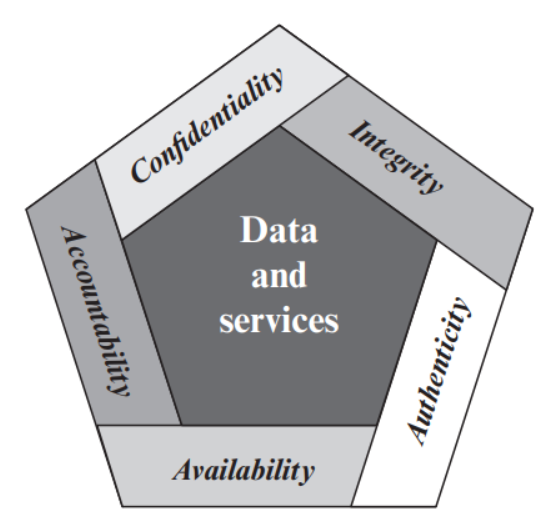
\includegraphics[width=\linewidth]{images/image-security.png}
    \caption{Essential Network and Computer Security Requirements.} \label{fig1}
\end{figure}

\subsubsection{Definicja kryterium oceny pod kątem skalowalności}

Czym jest skalowalność 

\begin{quote}
    "Scalability – the ability to work well when the load or the number of users increases – failure handling, concurrency of components, transparency and providing quality of service." ~\cite[p. 21]{coulouris2011distributed}
\end{quote}

W rozdziale 1 autorzy definiują pojęcie skalowalności jako 4 główne aspekty systemu: Controlling the cost of physical resources, Controlling the performance loss, Preventing software resources running out, Avoiding performance bottlenecks, strony 20-21, czyli Kontrola kosztów zasobów fizycznych, Kontrola utraty wydajności, Zapobieganie wyczerpywaniu się zasobów oprogramowania, Unikanie wąskich gardeł wydajności, dlatego mogę zdefiniować kryterium oceny pod kątem skalowalności jako:

\begin{enumerate}
    \item Wpływ na koszty zasobów fizycznych - to jak wzrostu obciążenia wpływa na koszty utrzymania sprzętu.
    \item Wpływ na wydajność - wydajność systemu w miarę wzrostu obciążenia.
    \item Wpływ na zasoby serwera - jak program wykorzystuje zasoby serwera w miarę wzrostu obciążenia.
    \item Unikanie wąskich gardeł wydajności - wiarygodność powstania wąskich gardeł w miarę wzrostu obciążenia systemu.
\end{enumerate}

\subsubsection{Definicja kryterium oceny pod kątem wersjonowania}

Za pomocą źródeł literaturowych oraz własnego doświadczenia zdefiniowałem kryteria oceny pod kątem wersjonowania jako:

% AI
\begin{enumerate}
    \item \textbf{Kompatybilność wsteczna} - Zapewnienie, że starsze wersje systemu lub komponentów nadal będą działały poprawnie, mimo wprowadzania nowych wersji. Kompatybilność wsteczna pomaga zapewnić funkcjonowanie istniejących systemów mikroserwisów w trakcie wprowadzania zmian i rozwoju systemu, pozwala przejść z kosztownych i bardzo skomplikowanych upgrade'ów systemu w całości za raz, a podzielić prace na mniejsze, łatwiejsze do zarządzania kawałki.
    \begin{quote}
        "APIs, like diamonds, are forever. Once you publish an API, you are more or less stuck with it, so it is critically important to design it well. When evolving an API, preserving backward compatibility is crucial to avoid breaking existing clients." ~\cite[p. 75]{bloch2018effective}
    \end{quote}
    
    \item \textbf{Łatwość migracji} - Prostota przejścia między wersjami, umożliwienie łatwego przechodzenia między różnymi wersjami plików lub interfejsów, aby dostosować się do zmian bez wprowadzania zakłóceń w pracy systemu. Możliwość zmniejszenia przestojów aplikacji w trakcie prac serwisowych i możliwość płynnego przejścia na nową wersję. Proste migracje przyspieszają proces rozwoju aplikacji i zmniejszają ilość błędów.
    \begin{quote}
        "When evolving an API, it is essential to provide a smooth migration path for clients. Deprecating old functionality rather than removing it immediately allows developers to transition gradually without breaking their systems." ~\cite[p. 78]{bloch2018effective}
    \end{quote}
    
    \item \textbf{Zarządzanie historią wersji} - Możliwość przechowywania i uzyskiwania dostępu do poprzednich wersji plików. Historia wersji pozwala programistom szybko i łatwo przywrócić poprzednią wersję w przypadku powstania błędu w nowej wersji. Pozwala na zmniejszenie utraty danych i niespójności w trakcie rozwoju aplikacji. Posiadanie historii wersji zapewnia to, że projekty pozostają łatwe w utrzymaniu i skalowalne.
    \begin{quote}
        "Effective version management is crucial for tracking changes over time, allowing teams to understand what was modified, when, and by whom. A well-maintained version history ensures accountability and facilitates rollback if necessary." ~\cite[p. 150]{rubin2012essential}
    \end{quote}
    
    \item \textbf{Śledzenie zmian} - Zdolność systemu do rejestrowania i monitorowania wszystkich zmian. Możliwość śledzenia zmian zapewnia to, że każda zmiana w systemie będzie zapisana, wspierając tym programistów w zrozumieniu problemów i błędów albo pozwalając cofnąć zmiany. Poprawia współpracę między zespołami, wykazując kto, kiedy i dlaczego wprowadzał zmiany, co zwiększa również odpowiedzialność. W branżach regulowanych prawem taka audytowalność systemu może być wymagana przez prawo.
    \begin{quote}
        "Tracking changes in source code is essential for understanding the evolution of a system. Without a proper change history, debugging, auditing, and maintaining software become significantly more difficult." ~\cite[p. 150]{rubin2012essential}
    \end{quote}
\end{enumerate}

\subsection{Ocena i porównanie metod współdzielenia kodu}

\subsubsection{Ocena wspówdzieleina kodu za pomocą Interface definition languages}

Ocena pod kątem komunikacji – zapewnia potrzebny poziom komunikacji, obiekty są generowane na podstawie języka definicji interfejsu (IDL) na etapie uruchamiania aplikacji. Dalej, w trakcie wykonywania logiki programu, takie obiekty mogą być używane przez program bez obciążenia wydajnościowego. Obiekty wygenerowane na podstawie plików IDL mogą być wykorzystane do komunikacji asynchronicznej, takich jak brokery wiadomości, jak również do wysyłania bezpośrednich zapytań między serwisami.

Metody zarządzania plikami idl w systemach : 

% AI
\begin{enumerate}
    \item SVN systemy takie jak, na przykład GIT - Rozwiązania posiada następujące korzyści: łatwe osiągnięcie wstecznej kompatybilności, ułatwienie osiągnięcia jednego źródła prawdy w systemie mikroserwisów, łatwiejsze zapewnienie tego, że wszystkie usługi korzystają z najnowszej wersji IDL. Do minusów rozwiązania możemy odnieść to, że system SVN może szybko stać wąskim gardłem w przypadku wykorzystania przez wiele zespołów, wymaga zarządzania i utrzymania.
    \item Dystrybucja za pomocą bibliotek - Kompilowanie plików IDL do współdzielonych bibliotek, i publikacja w współdzielonym repozytorium pakietów, na przykład Nexus. Do korzyści tego rozwiązania możemy odnieść łatwą integrację z procesami CI/CD, możliwość korzystania z wersjonowanych artefaktów bez bezpośredniej interakcji z surowymi plikami IDL oraz to, że różne języki programowania mogą wymagać różnych bibliotek, co zwiększa złożoność systemu.
    \item Podejście Monorepo - Przechowywanie wszystkich mikroserwisów i powiązanych z nimi plików IDL w jednym repozytorium, co zapewni, że wszystkie zespoły będą pracować na tej samej bazie kodu. Do korzyści tego rozwiązania możemy odnieść to, że pliki IDL w implementacjach usług są zawsze zsynchronizowane oraz to, że takie podejście upraszcza zarządzanie zależnościami, ponieważ cały kod przechowywany jest w jednym miejscu. Do wad podejścia mogę odnieść problemy ze skalowalnością, zwiększenie ilości kodu oraz to, że często wymaga narzędzi do zarządzania dużymi bazami kodu.
    \item Repozytoria z automatyczną synchronizacją - Repozytoria z automatyczną synchronizacją to specyficzny rodzaj repozytoriów, w których zmiany wprowadzone w głównym repozytorium są automatycznie propagowane do pozostałych subrepozytoriów. Dzięki temu każdy uczestnik projektu ma dostęp do wszystkich wersji kodu. Do zalet tego podejścia możemy zaliczyć możliwość scentralizowanego wymuszania wersjonowania oraz łatwy dostęp do wszystkich wersji plików. Do minusów możemy zapisać dość trudne utrzymanie oraz złożoność w zarządzaniu synchronizacją i konfliktami w repozytorium.
    \item IDL as a Service (IDLaS) - Przygotowana wcześniej usługa, która obsługuje pliki IDL na żądanie. Ta usługa może wersjonować, weryfikować i dostarczać pliki IDL. Do korzyści tego podejścia możemy odnieść dostęp na żądanie do plików IDL, możliwość dynamicznego wersjonowania. Do minusów możemy doliczyć to, że takie podejście wymaga zbudowania i utrzymania dodatkowej usługi w systemie oraz to, że komunikacja sieciowa może powodować opóźnienia w dostarczaniu plików IDL.
\end{enumerate}

Ocena pod kątem izolacji - ocena pod kątem izolacji zależy od implementacji zarządzania plikami IDL, dla każdego z powyżej opisanego podejścia dokonałem analizy.

Ze względu na to, że mamy wiele kryteriów oceny i wiele możliwych podejść do współdzielenia plików IDL, postanowiłem stworzyć tabelę porównawczą, która pomoże w czytelnym zaprezentowaniu wyników analizy.

Dane do porównania zostały zebrane z źródeł literaturowych. ~\cite{newman2015building} ,  ~\cite{kleppmann2017designing}
% AI 14%
\begin{table}[htbp]
    \centering
    \caption{Porównanie podejść do współdzielenia kodu w systemach mikroserwisów}
    \label{tab:comparison}
    \begin{tabularx}{\textwidth}{|>{\raggedright\arraybackslash}X|>{\raggedright\arraybackslash}X|>{\raggedright\arraybackslash}X|>{\raggedright\arraybackslash}X|>{\raggedright\arraybackslash}X|>{\raggedright\arraybackslash}X|}
    \hline
    \textbf{Kryteria} & \textbf{SVN/Git Systemy} & \textbf{Biblioteki} & \textbf{Podejście Monorepo} & \textbf{Repo z Auto-Synchro.} & \textbf{IDL as a Service (IDLaS)} \\
    \hline
    \textbf{Conflict Rate} &
    Wysoki: Merge konflikty są powszechne w przypadku wykorzystania przez kilkoma zespołami jednocześnie. Rozwiązanie takich konfliktów może być zasobochłonne &
    Umiarkowany: Konflikty są mniej powszechne, ale wciąż mogą wystąpić. &
    Niski: Zespoły pracują na tej samej bazie kodu, dlatego konflikty zdarzają się rzadko, mogą wystąpić w trakcie pracy na tej samej usłudze. &
    Umiarkowany: Konflikty mogą wystąpić, dlatego w przypadku gdy synchronizacja między usługami nie jest dobrze zarządzana. &
    Niski: Konflikty zdarzają się rzadko, dlatego, że IDL są dostarczane na żądanie a wersjonowanie jest wymuszane. \\
    \hline
    \textbf{Version Drift Occurrence} &
    Umiarkowana: Może wystąpić jeśli zespoły programistów nie aktualizują się do nowszej wersji regularnie. &
    Niski: Wiarygodność jest minimalna, ponieważ biblioteki są wersjonowane i dystrybuowane za pomocą odpowiednich narzędzi. &
    Niski: Bazy kodu w tym przypadku baza kodu jest synchronizowana co minimalizuje problemy z wersjonowaniem. &
    Umiarkowany: Problemy mogą wystąpić, jeśli synchronizacja nie jest dobrze utrzymana. &
    Bardzo Niski: Dynamiczne zarządzanie wersjami po stronie usługi zmniejsza wiarygodność problemów z wersjonowaniem. \\
    \hline
    \textbf{Build Failure Rate} &
    Wysoki: Błędy w trakcie kompilacji mogą wystąpić w przypadku niekompatybilnych usług. &
    Umiarkowana: Awarie zdarzają się rzadko, możliwe są z przypadku nieprawidłowych wersji zawartych w bibliotece. &
    Umiarkowana: Błędy w trakcie kompilacji zdarzają się rzadko, ze względu na synchronizację kodu. &
    Umiarkowana: Błędy w trakcie kompilacji zdarzają się rzadko, możliwe w przypadku niedysynchronizacji repozytorium. &
    Niska: Minimalne ryzyko błędów w trakcie kompilacji ze względu na wymuszaną synchronizację. \\
    \hline
    \textbf{Deployment Rollback Frequency} &
    Wysoka: Częste zmiany w plikach IDL mogą spowodować częste wycofanie zmian w trakcie wdrożenia. &
    Umiarkowana: Wycofania zmian w trakcie wdrożenia mogą wystąpić, jeśli wystąpią problemy z kompatybilnością wsteczną. &
    Umiarkowana: Wycofania zmian w trakcie wdrożenia są rzadsze ze względu na synchronizację, ale problemy mogą wystąpić. &
    Niska: Wycofania zmian w trakcie wdrożenia są rzadkie, automatyczna synchronizacja minimalizuje potrzebę wycofywania zmian. &
    Niska: Wycofania zmian w trakcie wdrożenia są rzadkie. Zarządzanie IDL na żądanie zmniejsza częstotliwość wycofywania. \\
    \hline
    \end{tabularx}
\end{table}

\newpage

Ocena pod kątem bezpieczeństwa:
% AI 15%
\begin{longtable}{|p{4cm}|p{4cm}|p{4cm}|}
    \caption{Porównanie SVN, bibliotek, Monorepo i IDLaS pod kątem bezpieczeństwa.} \\ 
    \hline
    \textbf{Kryteria} & \textbf{Zalety} & \textbf{Wyzwania} \\ \hline
    \multicolumn{3}{|c|}{\textbf{SVN }} \\ \hline
    Poufność & Zaawansowane mechanizmy kontroli dostępu wspierają w zapewnieniu poufności & Wymaga odpowiedniej dodatkowej konfiguracji \\ \hline
    Integralność & Pełna i przejrzysta historia zmian zapewnia integralność danych & Problemy z integralnością mogą wystąpić w przypadku, gdy zmiany nie zostaną prawidłowo zsynchronizowane \\ \hline
    Dostępność & Scentralizowane repozytorium dostępne z wielu lokalizacji & Awaria serwera centralnego może ograniczyć dostęp \\ \hline
    Autentyczność & Uwierzytelnianie użytkowników kontroluje dostęp do repozytorium & Nieprawidłowa konfiguracja uwierzytelniania może prowadzić do problemów z bezpieczeństwem \\ \hline
    Odpowiedzialność & Za pomocą uwierzytelniania można kontrolować dostęp do repozytorium & Proces przeprowadzenia audytu w systemie musi być prawidłowo skonfigurowany \\ \hline
    \multicolumn{3}{|c|}{\textbf{Dystrybucja za pomocą bibliotek (Nexus)}} \\ \hline
    Poufność & Uwierzytelnianie i mechanizmy kontroli dostępu pomagają chronić pliki IDL & Nieprawidłowa konfiguracja może prowadzić do nieautoryzowanego udostępniania \\ \hline
    Integralność & Kontrola wersji artefaktów zapewnia integralność & Brak wersjonowania może spowodować problemy \\ \hline
    Dostępność & Scentralne przechowywanie artefaktów zapewnia dla nich dostępność & Wymaga dodatkowej konfiguracji do prawidłowego działania \\ \hline
    Autentyczność & Mechanizmy podpisywania artefaktów pomagają w znalezieniu zaufanych źródeł & Wymaga prawidłowej konfiguracji \\ \hline
    Odpowiedzialność & Nie wszystkie rozwiązania zapewniają audyt i monitorowanie działań użytkowników & Właściwe logowanie zewnętrzne jest niezbędne do rozliczalności \\ \hline
    \multicolumn{3}{|c|}{\textbf{Podejście Monorepo}} \\ \hline
    Poufność & Scentralizowana kontrola dostępu pomaga poprawić bezpieczeństwo & Zarządzanie dostępem w dużych repozytoriach potrafi być skomplikowane \\ \hline
    Integralność & Scentralizowane zarządzanie zmianami pomaga w zapewnieniu spójności & Są różne wyzwania związane z synchronizacją w dużych zespołach \\ \hline
    Dostępność & Scentralizowane repozytorium umożliwia łatwy dostęp do treści repozytorium & Wymaga solidnie postawionej infrastruktury do użytku na dużą skalę \\ \hline
    Autentyczność & Kontrola dostępu na wyższym poziomie w organizacji pomaga w zapewnieniu bezpieczeństwa & Zarządzanie uprawnieniami w dużych zespołach jest trudne i może doprowadzić do błędów \\ \hline
    Odpowiedzialność & Scentralizowane procesy biznesowe umożliwiają pełne śledzenie zmian & W dużych organizacjach trudniej znaleźć odpowiedzialnego za błąd w rezultacie audytu \\ \hline
    \multicolumn{3}{|c|}{\textbf{IDL as a Service (IDLaS)}} \\ \hline
    Poufność & Bezpieczne punkty końcowe API z uwierzytelnianiem i szyfrowaniem zapewniają poufność & Wymaga konfiguracji bezpieczeństwa i stałego monitorowania dostępu \\ \hline
    Integralność & Systemy kontroli wersji i automatyczna dokumentacja mogą pomóc w zapewnieniu integralności zmian & Nieprawidłowe zarządzanie wersjami może prowadzić do problemów z integralnością \\ \hline
    Dostępność & Zapewnia wysoką dostępność dzięki automatycznemu zarządzaniu zasobami & Zależność od stabilnego połączenia sieciowego \\ \hline
    Autentyczność & Mechanizmy uwierzytelniania, autoryzacji i certyfikatów cyfrowych wspomagają uwierzytelnienie & Wymaga regularnego monitorowania systemu bezpieczeństwa \\ \hline
    Odpowiedzialność & Szczegółowe logi umożliwiają precyzyjne śledzenie zmian & Integracja z systemami zarządzania logami wymaga konfiguracji \\ \hline
\end{longtable}

Ocena pod kątem skalowalności:

Systemy bazujące na IDL, takie jak Protocol Buffers oraz Avro zazwyczaj serializują dane do kompaktowych formatów binarnych, to znaczy, że ilość danych, które trzeba przesłać przez sieć i przechowywać na dysku, jest minimalna. Dzięki temu koszt zasobów fizycznych jest minimalny i ma tendencję do pozostania niskim, nawet w przypadku wzrostu obciążenia. Wydajność systemu korzystającego z współdzielenia za pomocą IDL nie zależy od metody zarządzania plikami IDL, jak w powyższych przypadkach.

\begin{quote}
    "With efficient binary serialization formats, IDLs allow rapid encoding and decoding of messages. This efficiency is crucial for high-throughput systems where low latency is required. IDLs also facilitate cross-language interoperability without incurring significant performance penalties." ~\cite[p. 123]{kleppmann2017designing}
\end{quote}

Ocena pod kątem wersjonowania:

Na podstawie analizy źródeł literaturowych oraz doświadczenia własnego dokonałem analizy podejścia do współdzielenia kodu za pomocą plików IDL. W tym przypadku ocena pod kątem wersjonowania różni się w zależności od podejścia do zarządzania plikami IDL, dlatego dokonałem porównania dla każdego z podejść.

\begin{longtable}{|C{3cm}|C{9.1cm}|}
    \caption{Porównanie podejść do zarządzania kodem, wersjonowania i repozytoriami: Git, biblioteki, Monorepo i IDLaS.} \\
    \hline
    \textbf{Zaleta} & \textbf{Opis} \\
    \hline
    \endfirsthead

    \hline
    \textbf{Zaleta} & \textbf{opis} \\
    \hline
    \endhead

    \hline
    \endfoot

    \hline
    \endlastfoot

    \multicolumn{2}{|c|}{\textbf{1. SVN Systemy (Git)}} \\ \hline
    śledzienie zmian &
    \begin{itemize}
      \item Każda zmiana jest rejestrowana w postaci commitu z timestampem i informacjami wskazującymi autora.
      \item Rozgałęzianie i tagowanie umożliwiają izolowane przygotowanie paczki zmian i później oznaczanie stabilnych wersji.
      \item Pełna historia commitów umożliwia przeprowadzani audytów.
    \end{itemize} \\ \hline
    Rozgałęzianie i tagowanie &
    \begin{itemize}
      \item Rozgałęzienie pozwala zespołom na przygowtoanie nowych wersji oprogramowania w izolacji, nie prxerywając pracy innych zespołów.
      \item Tagi dają możliwości oznaczania stabilnych wersji, zapewniając łatwą identyfikację wersji gotowych do użytku.
    \end{itemize} \\ \hline
    Audytowalność &
    \begin{itemize}
      \item Pełna historia commitów jest zawsze przechowywana, co umożliwia audyty kodu.
      \item Zapewnia odpowiedzialnosc za wprowadzone zmniany i usprawnia współpracę w zespołów.
    \end{itemize} \\ \hline
    
    \multicolumn{2}{|c|}{\textbf{2. Biblioteki}} \\ \hline
    Wersjonowanie semantyczne &
    \begin{itemize}
      \item Artefaktom przypisywane są numery.
      \item Do każdej wersji dołączone są "Release notes".
      \item Repozytoria przechowują pełną historię wersji.
    \end{itemize} \\ \hline
    Dzienniki zmian &
    \begin{itemize}
      \item Do każdego wydania dołączona szczegółowa dokumentacja.
      \item Takie changelogi zmian zapewniają uporządkowaną historię modyfikacji,.
      \item Takie podejście zapewnia to przejrzystość śledzenia zmian.
    \end{itemize} \\ \hline
    Centralne repozytorium artefaktów &
    \begin{itemize}
      \item Centralne repozytorium przechowuje kompletną historię wersji.
      \item Dzięki temu zespoły mogą, w razie potrzeby, pobierać, porównywać i przywracać wcześniejsze stabilne wersje.
    \end{itemize} \\ \hline

    \multicolumn{2}{|c|}{\textbf{3. Podejście Monorepo}} \\ \hline
    Zunifikowany dziennik zmian &
    \begin{itemize}
      \item Wszystkie mikrserwisy w systemie i powiązane z nimi pliki IDL znajdują się w jednym repozytorium.
      \item Historia commitów zapewnia całościowy widok zmian.
    \end{itemize} \\ \hline
    Spójność &
    \begin{itemize}
      \item Wszystkie zmiany są wprowadzane do jednego repozytorium, co zapewnia synchronizację.
      \item Takie podejście minimalizuje ryzyko różnic w wersjach pomiędzy usługami.
      \item Spójne wersjonowanie poprawia stabilność systemu.
    \end{itemize} \\ \hline
    Łatwość cofanięcia &
    \begin{itemize}
      \item Scentralizowana historia ułatwia powrót do poprzedniego stabilnego stanu.
      \item Takie podejście ułatwia debugowanie i zwieększa stabilność systemu.
    \end{itemize} \\ \hline

    \multicolumn{2}{|c|}{\textbf{4. IDL as a Service (IDLaS)}} \\ \hline
    Zintegrowana kontrola wersji &
    \begin{itemize}
      \item Dostarczana usługa obejmuje wbudowaną kontrolę wersji.
      \item Dostarczana usługa daję dostęp do histoii wersji za pomocą API.
    \end{itemize} \\ \hline
    Automatyczna dokumentacja &
    \begin{itemize}
      \item IDLaS często udostępniają interfejsy webowe.
      \item Ze względu na to, że IDL jest udostępniane jako usługa, każdy użytkownik może uzyskać dostęp do historii wersji za pomocą API
    \end{itemize} \\ \hline

\end{longtable}

\subsubsection{Ocena wspówdzieleina kodu za pomocą bibliotek}

Ocena pod kątem komunikacji:

Pod kątem komunikacji podejście zapewnia potrzebny poziom komunikacji, obiekty są dodawane do projektu przez narzędzie do budowania projektów na etapie uruchamiania aplikacji, dalej w trakcie wykonania logiki programu takie obiekty mogą być użyte przez program bez żadnych obciążeń wydajnościowych. Obiekty wciągnięte z biblioteki mogą być użyte dla komunikacji asynchronicznej, takich jak brokery wiadomości, jak również dla wysłania bezpośrednich zapytań między serwisami.

Ocena pod kątem izolacji:

Zgodnie z wcześniej zaprezentowanymi kryteriami oceny, w przypadku oceny izolacji bibliotek, kryteria oceny są następujące: ocena pod kątem izolacji interfejsów, izolacji wersji oraz izolacji zależności.

Izolacja interfejsów: Dobrze ustrukturyzowana biblioteka izoluje skomplikowane elementy logiki od swoich użytkowników. Gdy są użyte prawidłowo, biblioteki pozwalają na zmianę lub aktualizację kodu przy minimalnym wpływie na kod wykorzystujący bibliotekę.

\begin{quote}
    "A well-designed library or SDK isolates its implementation details from the user." ~\cite[p. 75]{Essential}
\end{quote}

Izolacja wersji: Biblioteki zazwyczaj używają semantycznego wersjonowania za pomocą nazwy. Przejrzysta historia wersji umożliwia deweloperom odpowiednie zarządzanie zależnościami. Przy odpowiedniej izolacji wersji wiele wersji biblioteki może współistnieć i być używane jednocześnie, ułatwia to proces stopniowej migracji.

\begin{quote}
    "Versioning APIs and libraries carefully ensures that changes can be introduced gradually." ~\cite[p. 172]{fowler2012patterns}
\end{quote}

Izolacja zależności: Biblioteki często zależą od innych bibliotek, w przypadku gdy zależności nie są prawidłowo izolowane mogą prowadzić do konfliktów i innych problemów. Dobre praktyki zarządzania zależnościami pomagają zapewnić, że zależności biblioteki nie będą miały negatywnego wpływu na aplikację.

\begin{quote}
    "Dependencies should be isolated to minimize their impact on the main application." ~\cite[p. 218]{martin2008clean}
\end{quote}

Ocena pod kątem bezpieczeństwa:

Zgodnie z wcześniej zaprezentowanymi kryteriami oceny, w przypadku oceny bezpieczeństwa bibliotek kryteria oceny są następujące: Poufność, Integralność danych, Dostępność, Autentyczność, Odpowiedzialność.

Poufność: Biblioteki, które są wykorzystywane do przetważania poufnych danych muszą pochodzić z sprawdzonych źródeł i ciągle aktualizowane, aby zapobiec utracie danych.

% AI
\begin{quote}
    "Ensuring that libraries handling sensitive information are sourced from reputable channels and regularly updated is critical to maintaining confidentiality throughout an application." ~\cite[p. 82]{Essential}
\end{quote}

Integralność danych: Biblioteki często korzystają z sum kontrolnych, certyfikatów, podpisów cyfrowych aby mieć pewność, że przetwarzane dane pozostają bezpieczne.

\begin{quote}
    "The integrity of a library is maintained through rigorous testing and the use of cryptographic measures that detect any unauthorized changes to the code or data it processes." ~\cite[p. 84]{Essential}
\end{quote}

Dostępność: Dostępność może zostać naruszona, jeśli biblioteki zewnętrzne będą niedostępne, lub wewnętrzne w przypadku awarii narzędzia do zarządzania bibliotekami. Dlatego ważne jest wykorzystanie menedżerów zależności które są zaufane.

\begin{quote}
    "By leveraging modern dependency management tools and regularly updating libraries, developers can mitigate risks to availability due to deprecated or unsupported components." ~\cite[p. 85]{Essential}
\end{quote}

Autentyczność: W przypadku bibliotek jest zapewniana za pomocą sprawdzenia jej pochodzenia za pomocą podpisów cyfrowych i sum kontrolnych dostarczonych przez wydawcę. Zapobiega to ryzyku włączenia wykonania złośliwego kodu po stronie klienta biblioteki.

\begin{quote}
    "Authenticating libraries through digital signatures and secure distribution channels is essential to ensuring that only verified, unmodified code is used in production environments." ~\cite[p. 87]{Essential}
\end{quote}

Odpowiedzialność: W przypadku bibliotek przejrzysta historia może zostać zapewniona za pomocą menedżerów pakietów, które umożliwiają śledzenie pochodzenia zmian. Wspomaga to w zapewnieniu odpowiedzialności w przypadku problemów.

\begin{quote}
    "A well-documented version history is indispensable for accountability, as it enables developers to trace and audit every modification made to a library over time." ~\cite[p. 88]{Essential}
\end{quote}

Ocena pod kątem skalowalności:

Libraries are generally optimized for specific tasks within one language. However, if a library is not designed for high-concurrency environments, it may require additional hardware resources as the load increases. For example, intensive data processing libraries may consume more memory or CPU when dealing with large datasets. Supporting Idea: Studies on computational efficiency often note that non-optimized libraries can become bottlenecks under heavy load, leading to increased physical resource costs.

\begin{quote}
    "Non-optimized libraries can quickly become bottlenecks in high-concurrency environments, forcing systems to consume additional CPU and memory resources as load increases." ~\cite[p. 192]{fowler2012patterns}
\end{quote}

Ocena pod kątem wersjonowania:

\begin{quote}
    "When a data format or schema changes, … careful management of schema evolution is required to ensure that old and new versions can coexist. This is best achieved by maintaining a structured version history that records every change in the schema in a clear, traceable manner." ~\cite[p. 111]{kleppmann2017designing}
\end{quote}

Ustrukturyzowana historia wersji:

\begin{quote}
    "APIs, like diamonds, are forever. Once you publish an API, you are more or less stuck with it; hence, maintaining a clear, structured version history through semantic versioning is critical for ensuring that developers know exactly when breaking changes occur." ~\cite[p. 75]{Essential}
\end{quote}

text

\begin{quote}
    "When an API change turns out to be problematic, having a stable version available through semantic versioning allows developers to quickly roll back to a previous release and restore system stability." ~\cite[p. 75]{Essential}
\end{quote}

text

\begin{quote}
    "Inadequate versioning can lead to subtle incompatibilities, resulting in data inconsistencies that are difficult to debug. Hence, maintaining strict backward compatibility is crucial to avoid such pitfalls." ~\cite[p. 75]{Essential}
\end{quote}

\subsubsection{Ocena wspówdzieleina kodu za pomocą SDK}

Ocena pod kątem komunikacji: zapewnia potrzebny poziom komunikacji, mechanizm współdzielenia jest podobny do biblioteki, tak samo jak w przypadku biblioteki obiekty są dodawane do projektu przez narzędzie do budowania projektów na etapie uruchamiania aplikacji, dalej w trakcie wykonania logiki programu takie obiekty mogą być użyte przez program bez żadnych obciążeń wydajnościowych. Obiekty wciągnięte z biblioteki mogą być użyte dla komunikacji asynchronicznej takich jak brokery wiadomości jak również dla wysłania bezpośrednich zapytań między serwisami.

Ocena pod kątem izolacji: 

Zgodnie z wcześniej zaprezentowanymi kryteriami oceny, w przypadku oceny izolacji SDK kryteria oceny są następujące: ocena pod kątem izolacji interfejsów, izolacja wersji, izolacja zależności. Jednak są one trudniejsze w projektowaniu i wymagają ostrożności w trakcie zarządzania.

\begin{quote}
    "SDK isolates its implementation details from the user, allowing developers to interact with the API without needing to understand its inner workings." ~\cite[p. 75]{Essential}
\end{quote}

Izolacja wersji: W przypadku SDK, które agregują kilka bibliotek i narzędzi, muszą zarządzać wersjonowaniem wszystkich zawartych komponentów. W idealnym przypadku zestaw SDK jest zaprojektowany tak, aby nowe dodane wersje były kompatybilne wstecz, umożliwiając klientom działanie bez natychmiastowych zmian.

Izolacja zależności: SDK często zawierają wiele bibliotek w sposób, co oznacza, że często zarządzają dużą ilością zależności. Izolowanie tych zależności jest krytyczne, aby uniknąć konfliktów.

\begin{quote}
    "...ensuring that dependencies can be replaced without affecting the core business logic" ~\cite[p. 218]{martin2008clean}
\end{quote}
% AI
Ocena pod kątem bezpieczeństwa: 

Zgodnie z wcieśniej zaprezentowanymi kryteriami oceny, w przypadku oceny bezpieczeństwa bibliotek kryteria oceny są następujące: Poufność, Integralność danych, Dostępność, Autentyczność, Odpowiedzialność

Poufność: SDK w przypadku polączenia wielu narzędzi i bibliotek, muszą zapewnić, że wszystkie zawarte komponenty przestrzegają ścisłych zasad kontroli dostępu. Zmniejsza to ryzyko nieautoryzowanego ujawnienia danych.

\begin{quote}
    "SDKs, when integrated with stringent access controls and privacy policies, help shield sensitive data from unauthorized access, thus preserving confidentiality across all integrated modules." ~\cite[para 4]{azure2020}
\end{quote}

Integralność danych: SDK wymaga, aby były one kompleksowo testowane, aby zapewnić, że zmiany nie naruszą integralności danych. Różne frameworki do testowania bezpieczeńswa SDK pomagają w wykrywaniu wszelkich podatności po modyfikacji.

\begin{quote}
    "Robust testing frameworks within SDKs are critical for maintaining integrity, ensuring that updates do not inadvertently alter data structures or application behavior." ~\cite[para 5]{azure2020}
\end{quote}

Dostępność: SDK muszą być zaprojektowane tak, aby działały zawszę, nawet przy dużym obciążeniu. 

\begin{quote}
    "The modular and redundant design of well-architected SDKs contributes significantly to system availability, ensuring that critical services remain accessible even under peak loads." ~\cite[para 6]{azure2020}
\end{quote}

Autentyczność: Autentyczność w przypadku z SDK może zostać zapewniona za pomocą weryfikacji dostawców i stosowanie środków kryptograficznych do walidacji ich komponentów. Warto dokonywac tachi wdziałań aby zapobiec wykonaniu złośliwego kodu w naszym systemie.

\begin{quote}
    "Verifying the authenticity of an SDK via cryptographic signatures and secure distribution channels is vital to ensure that the components used are genuine and have not been tampered with." ~\cite[para 7]{azure2020}
\end{quote}

Odpowiedzialność: SDK zazwyczaj posiadają przeróżne mechanizmy zarządzanie wersjami. Takie metody zarzadzania wersjami umożliwia deweloperom śledzenie pochodzenia wszelkich zmian lub problemów. Pomaga to zapełnić odpowiedzialność programistów za przygotowane zmiany.

\begin{quote}
    "Comprehensive logging and version tracking in SDKs provide the necessary audit trails that hold developers accountable for every change made, thereby ensuring that any issues can be traced back to their origin." ~\cite[para 7]{azure2020}
\end{quote}

Ocena pod kątem skalowalności:

SDK zazwyczaj zawierają wiele narzędzi czy komponentów Ta kompleksowość oznacza, że upraszczają dewelopment, mają tendencję do wyższego zużycia zasobów pamięci i procesora w porównaniu z, na przykład, IDL. Róznbe raporty dotyczące skalowania aplikacji w chmurach podkreślają, że SDK mogą powodować dodatkowe obciążenie na środowiskach z dużym obciążeniem.

\begin{quote}
    "SDKs, though beneficial for rapid development by bundling multiple tools, tend to impose a higher baseline resource consumption, especially under high-load production scenarios." ~\cite[para 3]{azure2020}
\end{quote}

\begin{quote}
    "Third-party SDKs can significantly increase memory and CPU usage, becoming a notable overhead in environments with high concurrent demands." ~\cite[p. 4]{ahmed2019impact}
\end{quote}

Ocena pod kątem wersjonowania:

SDK mogą zawirać wiele bibliotek i narzędzi, z których każde może nieć własną historię wersji. Wersjonowanie SDK może być  złożone, ponieważ musi odzwierciedlać zmiany we wszystkich wewnętrznych komponentach. Prowadzi to do bardziej zawożonej historii wersji, która wymaga dovbrej  dokumentacji i koordynacji.

\begin{quote}
    "SDKs encapsulate multiple interdependent modules. As a result, maintaining a structured version history across all components is challenging but essential in order to manage compatibility and coordinate upgrades effectively." ~\cite[para. 3]{azure2020}
\end{quote}

Przywracanie kodu do stabilnej wersji: Wycofywanie zmian w przypadku SDK może być trudnym, ponieważ SDK  może integrowac wiele komponentów. Ta złożoność może sprawić, że wycofywanie jest bardziej czasochłonne i podatny na błędy, jeśli nie jest zarządzany prawidłowo.

\begin{quote}
    "SDKs, by virtue of bundling several interdependent tools and libraries, require a coordinated rollback mechanism to ensure that all components revert to a stable, compatible state. This adds complexity compared to single-module libraries or IDL files." ~\cite[para. 3]{azure2020}
\end{quote}

Utrata danych i niespójność: SDK są narażone na większe ryzyko wewnętrznych niespójności i problemów w przypadku gdy moduły są aktualizowane asynchronicznie, może to doprowadzić do błędów, które mogą spowodować utratę danych lub uszkodzenie danych, jeśli nie są w odpowiedni sposówb zarządazane zarządzane.

\begin{quote}
    "The interdependencies within an SDK mean that even small version mismatches can lead to significant inconsistencies or data loss, making rigorous testing and coordinated versioning critical." ~\cite[para. 3]{azure2020}
\end{quote}

\subsubsection{Ocena wspówdzieleina kodu za pomocą API}

Ocena pod kątem komunikacji: 

\subsubsection{Ocena wspówdzieleina kodu za pomocą ServerLess}

\subsection{Opis części praktycznej}

Jaką część praktyczną mojej pracy magisterskiej przygotowałem aplikację webową, która : 
Składa się z dwóch części, back endowej i front endowej 
Głównym celem napisania aplikacji jest wprowadzenie nowego podejścia do współdzielenia kodu - współdzielenie za pomocą technologii serwer less. Aplikacja wspiera deweloperów korzystających z technologii serwer less, zmniejsza wady tego rozwiązania natomiast dając możliwość skorzystania z mocnych stron tej technologii.  

Czym jest technologia Serverless?

Serverless to nowoczesny model wykonywania obliczeń w chmurze, w którym dostawcy chmury automatycznie obsługują aspekty infrastruktury, takie jak zarządzanie serwerem oraz skalowanie zasobów. Zamiast zarządzać serwerami fizycznymi lub wirtualnymi, programiści mogą skupić się się wyłącznie na pisaniu kodu. Termin „serverless” nie oznacza że niema fizycznych serwerów, ale, że zarządzanie serwerem jest oderwane od użytkowników. W architekturach serverless wdrażamy do chmury funkcje zamiast całych aplikacji, a dostawca chmury jest odpowiedzialny za zarządzanie kodem, skalowanie i utrzymywanie tych funkcji. Są one też często nazywane Function-as-a-Service (FaaS).

Przykłady platform server less dostępnych w 2025 roku:

\begin{enumerate}
    \item AWS Lambda - Usługa, która umożliwia uruchamianie kodu bez zarządzania serwerami. AWS Lambda automatycznie skaluje aplikację, daje mozliwość uruchamiać kod po wyłowamiu odpowiednego zdarzenia.
    \item Azure Functions - Usługa świadczona przez Microsoft Azure, która umożliwia uruchamianie funkcji w chmurze, z automatycznym skalowaniem.
    \item Google Cloud Functions - Usługa świadczona przez Google Cloud, umożliwia uruchamianie kodu po wyłowamiu odpowiednego zdarzeniaw w Google Cloud lub w odpowiedzi na żądanie HTTP.
    \item IBM Cloud Functions - Usługa oparta na Apache OpenWhisk, obsługuje wykonywanie funkcji w różnych językach.
\end{enumerate}

\subsubsection{Ogulny opis aplikacji}

Za pomocą  przygotowanej przeze mnie aplikacji webowej wykonuję nastepujace czynności:

\begin{enumerate}
    \item Akceptuję i sprawdzam kod, który chcesz podzielić za pomocą technologii serverless. Jeśli coś nie gra w czasie sprawdzania, powiem ci, co masz zrobić, żeby skończyć to sukcesem.
    \item Automatycznie przygotowuję kod do wrzucenia na Amazon Lambda (w przyszłości może dać ci opcję wyboru innej platformy, jak na przykład Azure Functions).
    \item Automatycznie wrzucam kod na platformę Serverless, po chwili będzie od razu dostępny.
    \item Zapisuję kod w bazie danych, żebyś mógł go użyć później; będziesz miał widok na listę wszystkich wrzutków kodu.
    \item Możesz edytować i ponownie wrzucić kod z tej listy.
    \item Możesz wyszukać kod po opisie.
    \item Dodaję wersjonowanie kodu.
    \item Automatycznie przygotowuję pliki IDL, które są fajne do wykorzystania, gdy kod jest wywoływany na IDL.
    \item Przechowuję te pliki IDL i możesz je udostępnić, żeby inni członkowie zespołu mogli współdzielić ten kod.
\end{enumerate}

\subsubsection{Opis aplikacji back-end}

Używane technologie
Java: Język do napisania backendu
Spring Boot: Narzędzie które ułatwia tworzenie aplikacji w Javie
Maven: Automation templat, które automatyzuje tworzenie procedur śledzenia zależności projektu, kompilacji projektów w inteligentny sposób.
AWS Lambda: To jest obliczenie ludzi, które pożycza używanie serwerów, ale jednocześnie opiekunów, mogą tu pokazić i uruchomić kod bez konieczności wdrażania lub zarządzania serwerami
Protobuf: Jest to jezyk IDL do szybkiego kodowania i dekodowania obiektów DTO.
Jackson: Jeden z najsłynniejszych warz z ferajny do niglowania JSON-ów, jak również konwertowania wejście wyjścia na obiekty DTO itp w drugą stronę.
Ogólny opis:
Ta aplikacja jest częścią aplikacji webowej, która odpowiada za następujące wdizłania:
Odbiera kod jako dane wejściowe użytkownika: Akceptuje kod od użytkownika za pośrednictwem żądań HTTP.
Weryfikuje kod: Spawdza że otrzymany kod spełnia wymagane standardy i format.
Automatycznie wdraża kod jako funkcję Lambda: wdraża sprawdzony kod jako funkcję AWS Lambda.
Generuje pliki .proto: tworzy pliki .proto na podstawie kodu wejściowego, które mogą być używane do generowania obiektów DTO do komunikacji z wdrożoną funkcją Lambda.

\subsubsection{Opis aplikacji front-end}

Aplikacja front-endowa została przygotowana przy użyciu JavaScript, React i npm.
React to popularna biblioteka JavaScript do tworzenia aplikacji front-endowych, w szczególności aplikacji jednostronicowych, w których można tworzyć komponenty interfejsu użytkownika wielokrotnego użytku.
Npm (Node Package Manager) służy do zarządzania zależnościami i skryptami projektu.

Aplikacja jest zbudowana przy użyciu komponentów React, co umożliwia modułowy kod który możnz uźywać wielokrotmie. Każdy komponent reprezentuje część interfejsu użytkownika.

Ogólny opis:
Ta aplikacja jest częścią aplikacji webowej, część font-endowa jest odpowiedzialna  za następujące działania:
Przyjmowanie kodu, który uzytkownik chce wspówdzielić, a następnie wysyłanie go do serwera back-endowego.
Weryfikacja tego, czy kod spełnia wymagane standardy i formatowanie.
Wyświetlanie użytkownikowi wyników walidacji.
Możliwość przeglądania, edytowania i usuwania kodu, który został wcześniej zapisany i wdrożony w AWS Lambda.
Możliwość wyszukiwania wdrożonego kodu, używając jego opisu i nazwy.
Wsparcie wersjonowania kodu w celu śledzenia zmian lub przywracania poprzednich wersji.
Udostępnianie plików .proto: aplikacja front-end udostępnia użytkownikom wygeneroane pliki .proto, których uźytkownicy mogą użyć do generowania obiektów DTO dla komunikacji z wdrożoną funkcją Lambda.

\subsection{Podsumowanie}

\nocite{*}

\listoftables

\listoffigures

\bibliographystyle{plain}
\bibliography{thesisbibliography}

\section{Appendices}

\subsection{Sample Code}
\subsection{Sample Data}

\end{document}